\chapter{Design}
\label{design}
The literature has shown us that machine learning methods can be useful in generating feedback for students, and this can be combined with a visual display for intuitive understanding. The first design decisions to be made is the language and libraries to be used when writing the program.
\section{Language and Tools}
Two languages are immediate possibilities for implementation: Java\cite{java_site} and Python\cite{python_site}. Java because I had the most experience with Java, and some parts of Infandango were written in Java. Most of Infandango was, however, written in Python with I had also had some experience. Due to the emphasis the project has on machine learning, R\cite{r_site} was another approriate language. 
The final decision was to use Python with scikit-learn\cite{scikit_site} and pybrain\cite{pybrain_site} libraries: this provides the simplest integration with Infandango (since the parts with which this will need to be integrated are written in Python) and the libraries provide a variety of machine learning methods.

\section{Proposed Design}
A model is created using an approriate machine learning method. The method will be applied to data which has been stored and anonymised from a previous year in which the course was run. 
\subsection{Model}
The Khan Academy model is built based on one assumption: a user can always \emph{generate another example} and it will be of the \emph{same type}. These are two qualities which Infandango does not share. Infandango has a preset number of manually written exercises and they are not grouped \emph{strictly} by similarity. The first proposed model was to take the average for each week and use those averages as features for the model and the next week's average as the class. There are however some problems with this model:

\begin{itemize}
\item The semester has 8 weeks worth of exercises. If all 7 weeks are used as a feature and the score for week 8 is predicted then the user would not receive any feedback until the last week. If feedback is to be generated for each week then a separate model needs to be trained for each week: one model where there is only 1 week of evidence and week 2 is predicted, another where there are 2 weeks of evidence and week 3 is predicted and so on. Neither of these options are desirable.
\item Even after 3-5 weeks there would only just be enough data to start getting reasonable results CITE HERE % CITE HERE graph, even though it is for later model
\item Grouping data like this means we have a lot less training examples
\end{itemize}

A similar alternative to this model is to treat each question within a week separately, giving the model a much larger dimensionality. Although this does remove the latter two problems, the first problem still remains. This also raises the likelihood of data being missing for a feature (it is more common for a student to miss one exercise within a week than the whole week).
\\
Both of these models have been working with the assumption that we want to learn something about \emph{specific} questions. So if, for example, a question was particularly hard then the model might be able to learn that it should predict lower scores for that question. However, we have seen the difficulties that these models incur. For this reason a much simpler model was created. The model has \textit{\textbf{N}} features, each a percentage. Each feature represents a score from the corresponding previous question. The class is the score for the \textit{\textbf{N+1}} problem, so when a user is using the system it will try to predict their next score given their previous \textit{\textbf{N}} scores. This creates a moving window of previous scores, with each feature simply being \emph{a question} rather than, for example \emph{week 3, question 2b}.

\subsubsection{Unexplored Alternatives}
There are many unexplored possibilities for other features like a weighted moving average or the number of problems unfinished. With this project it was important to complete the system quickly so that user tests can be done over a period of weeks. Other possibilities for features and other learning methods can be explored in later projects.

\subsubsection{Training the model}
Django is used to retrieve the training data from the anonymised data from a previous year. This data is filtered into groups of \textit{\textbf{N+1}} consecutive results, with the final result being the class. For each set of \textit{\textbf{K}} results \textit{\textbf{K-N}} sets of results are created. This provides the machine learning methods with a lot more training data than alternative models.
\\%CAN ADD MORE HERE ABOUT TESTING OTHER RATIOS 
%can also talk about r2 scores
In order to decide which learning method to use sci-kit learn's cross validation method splits the data into training and testing sets, with a testing size of 20\%. Different machine learning methods were then trained on this data and tested by comparing their R2 scores. In Figure \ref{fig:comparison} it can also be seen that these tests are done multiple times over different values of \textit{\textbf{N}}. The highest accuracy is obtained by Logistic Regression at \textit{\textbf{N}} = 4. Logistic Regression is also the most consitent of the methods, thus making it the most appropriate choice.

\begin{figure}[p]
\centering
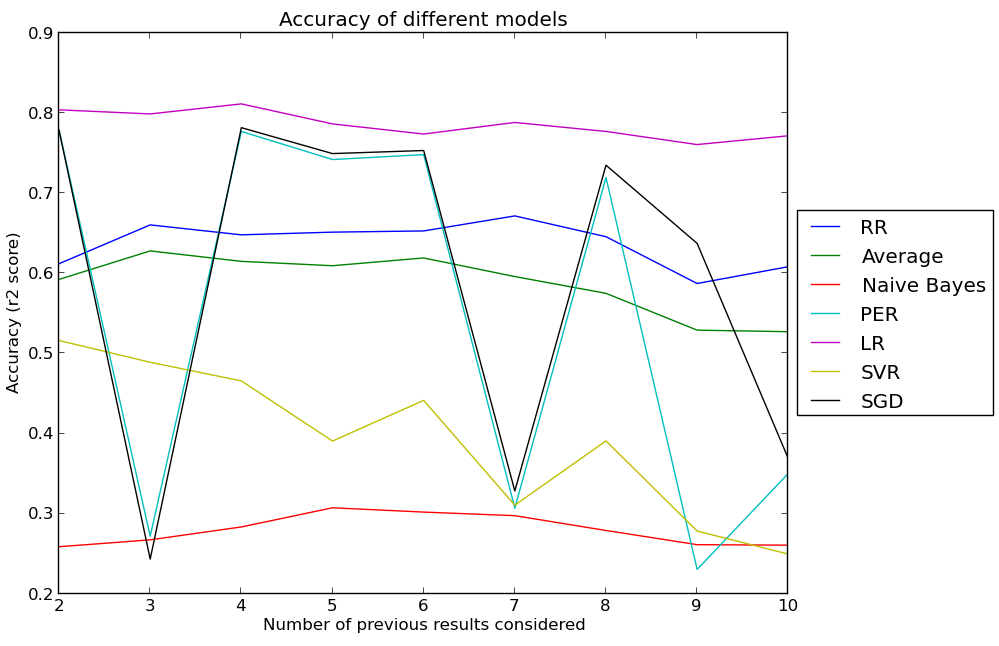
\includegraphics[width=1\textwidth]{comparison.png}
\caption{Comparison of different machine learning methods comparing their accuracy against the number of previous exercises considered}
\label{fig:comparison}
\end{figure}

%\subsubsection{Calibration}

\subsection{Visualising the results}

\section{Integration with Infandango}
